\documentclass[12pt, letterpaper]{article}
\usepackage{graphicx}
\graphicspath{{images/}}

\title{CCE5225 - Assignment 1 \\
\large MiniBooNE particle identification \\ signal/background classification}
\author{Sultan Dayani}
\date{December 2022}
\begin{document}
\maketitle
\pagebreak

\textgreater{Comment on whether the performance changes significantly amongst different hyperparameter values for each model.}
\\

\begin{tabular}{|c c c|}
\hline
HL Size & Mean Fit Time & Mean Score \\ [0.5ex] 
\hline
(10,) & 99.88s & 0.927113 \\
\hline
(20,) & 100.26s & 0.931188 \\
\hline
(30,) & 74.61s & 0.933052 \\
\hline
(40,) & 376.35s & 0.935090 \\
\hline
(50,) & 163.39s & 0.933744 \\ 
\hline
\end{tabular}

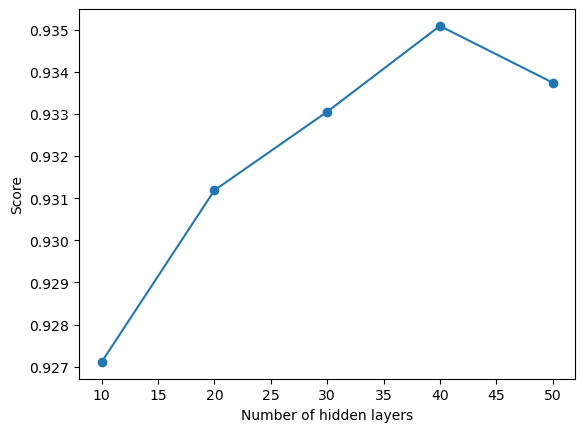
\includegraphics[width=0.6\textwidth]{1hiddenlayer_scores.png}

\textgreater{Report the time required for training, the set of hyperparameters which were tested, and the final per-class accuracies achieved on the unseen test set (in the form of a confusion matrix).}
\\

\textgreater{Comment on the performance of each model, and provide an explanation as to why you believe the highest performing model gave the best results.}




\end{document}